%%%%%%%%%%%%%%%%%%%%%%%%%%%%%%%%%%%%%%%%%%%%%%%%%%%%%%%%%
%%%%%%%%%%%%%%%%%         ANTECEDENTES              %%%%%%%%%%%%%%%%%%%%%%
%%%%%%%%%%%%%%%%%%%%%%%%%%%%%%%%%%%%%%%%%%%%%%%%%%%%%%%%%


\chapter{Resultados}
\label{chap:results}

\chapterintro{En este capítulo, se muestran los resultados obtenidos a lo largo de esta Tesis Doctoral en forma de publicaciones indexadas en el \textit{Journal Citation Reports} (JCR). En conjunto, dan respuesta a los objetivos enumerados en el capítulo anterior.}

Este capítulo inicia con un primer trabajo \cite{paper1} donde se analizan datos del microbioma fecal de pacientes con SM o DT2 para identificar taxones diferenciales. Posteriormente, en el segundo trabajo \cite{paper2}, se avanza hacia el campo predictivo, aplicando una metodología de ML para evaluar el potencial del microbioma en el diagnóstico temprano de DT1. Finalmente, el tercer trabajo \cite{paper3} analiza el microbioma vaginal en el contexto de la VB para caracterizar mejor los fenotipos, mejorar el subtipado y así encontrar asociaciones con el tratamiento. La Figura \ref{fig:papersGA} ofrece un resumen gráfico que sintetiza estas tres publicaciones.


\begin{figure}[h]
    \centering
    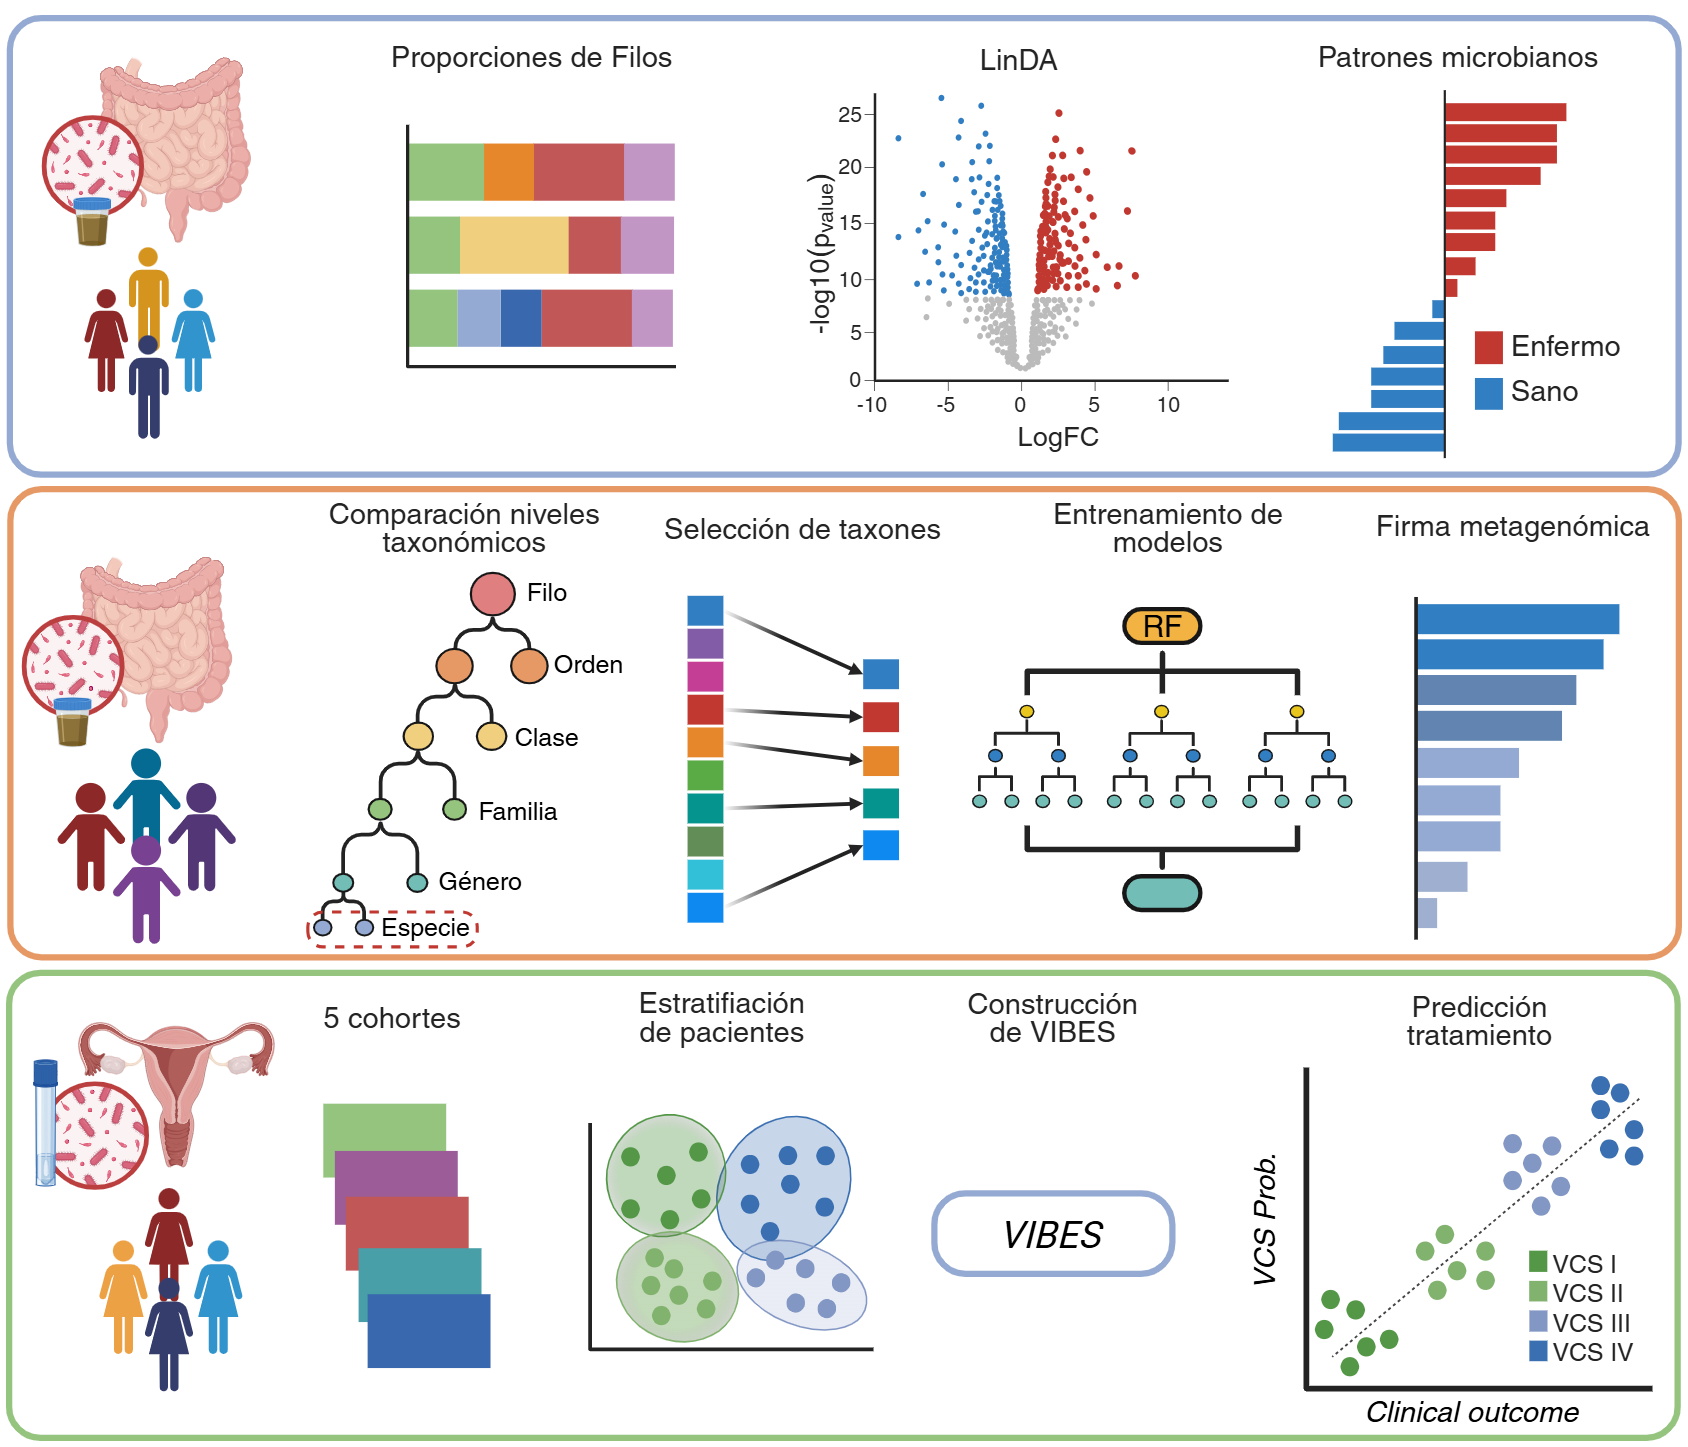
\includegraphics[width=\textwidth]{img/results/GA.png}
    \caption[\textit{Abstract} gráfico de las 3 publicaciones]{\textbf{\textit{Abstract} gráfico de las 3 publicaciones que conforman la Tesis Doctoral.} El primer trabajo \cite{paper1} analiza el microbioma intestinal en el contexto de SM y DT2. En el segundo trabajo \cite{paper2} se estudia el microbioma instestinal en infantes sanos y con DT1. Finalmente en el tercer trabajo \cite{paper3} se estudia el microbioma vaginal asociado a VB. Imagen creada con BioRender \cite{biorender2025}.}
    \label{fig:papersGA}
\end{figure}



\section{Búsqueda de patrones microbianos característicos de enfermedades metabólicas}


El incremento global de enfermedades metabólicas complejas como SM y DT2 destaca la necesidad urgente de comprender sus orígenes y mecanismos subyacentes \cite{saklayen2018global, zimmet2016diabetes}. Una línea prometedora de investigación se centra en el microbioma intestinal, dado su papel potencial en la regulación metabólica. Los desequilibrios en la composición del microbioma podrían ser fundamentales en la patogénesis de estas enfermedades al influir en factores como la inflamación y la resistencia a la insulina. Esta investigación se inspira en la posibilidad de que el análisis del microbioma pueda ayudar a identificar biomarcadores diagnósticos. Con esta motivación, este estudio se diseñó para identificar taxones con abundancias diferenciales que pudieran servir como biomarcadores en estas patologías, utilizando para ello la cohorte del proyecto IBEROBDIA \cite{IBEROBDIA_project}.

Este trabajo parte de dos esquemas de comparación: por un lado, individuos sanos frente a pacientes con SM; y por otro, una clasificación más detallada que distingue entre individuos sanos, prediabéticos y aquellos con DT2. El estudio del SM y DT2 desde perspectivas diferenciadas permite un análisis más preciso del impacto que pueden tener en el microbioma intestinal. El estudio del SM se caracteriza por su naturaleza como conjunto de factores de riesgo que predicen un mayor desarrollo hacia condiciones más graves, como DT2. Estudiar directamente los efectos del SM facilita la identificación de cambios microbianos que podrían ser utilizados como señales tempranas o indicadores de riesgo. Por otro lado, evaluar DT2 desde un punto de vista gradual (desde individuos sanos, pasando por prediabéticos, hasta diabéticos) ofrece una visión detallada de cómo los desequilibrios en el microbioma se desarrollan a lo largo del proceso de la enfermedad. Este enfoque diferencial no solo ayuda a identificar patrones específicos de disbiosis asociados a cada etapa, sino que también permite explorar posibles intervenciones y respuestas del microbioma a lo largo del avance de la enfermedad.

En primera instancia, se realizó un análisis exploratorio considerando las abundancias relativas a nivel de filo, así como la diversidad \textit{alfa} y \textit{beta}. Posteriormente, se empleó LinDA \cite{zhou2022linda} para analizar las abundancias relativas a nivel de género y especie. Los resultados de este trabajo indican que, a nivel de filo, es posible hallar indicadores asociados a ambas patologías. En particular, la relación Bacteroidetes/Firmicutes muestra variaciones relevantes y, en el caso de DT2, se observa un enriquecimiento de Actinobacteriota. En el caso del SM, se identifican varios taxones del género \textit{Blautia} que están sobrerrepresentados en los pacientes que sufren de este síndrome. En cuanto a la diabetes, se observa cómo taxones del género \textit{Bifidobacterium} están enriquecidos en pacientes sanos y cómo el taxón \textit{Dorea} (a través de \textit{Dorea longicatena}) está considerablemente sobrerrepresentado en los pacientes prediabéticos y diabéticos.

Los resultados obtenidos indican que los cambios en el microbioma intestinal están claramente asociados con SM y DT2, lo que refuerza hallazgos previos sobre la relación entre los organismos microbianos y estas patologías \cite{valdes2018role, lynch2016human, gurung2020role}. Sin embargo, nuestro trabajo ha identificado taxones que no han sido destacados en la literatura actual, como \textit{Parabacteroides merdae}, \textit{Lachnospiraceae GCA-900066575} y \textit{Defluviitaleaceae UCG-011}, lo que sugiere la necesidad de explorar otros géneros y/o especies que puedan estar asociadas con la enfermedad. Aunque existe la posibilidad de que algunos de los taxones identificados no tengan un efecto causal, podrían proporcionar información valiosa sobre la enfermedad como indicadores de diagnóstico.

El código fuente para reproducir todos los análisis, junto con la documentación, está disponible en GitHub (https://github.com/MALL-Machine-Learning-in-Live-Sciences/IBEROBDIA) y Zenodo (https://doi.org/10.5281/zenodo.14051704). Además, los datos brutos y los datos clínicos están disponibles en formato phyloseq en Figshare (https://doi.org/10.6084/m9.figshare.26063020.v1).

Fui coautor principal del trabajo liderando la parte computacional del mismo. Realicé el preprocesado y los análisis de los datos, construí las figuras y las tablas, y escribí el manuscrito. La información de participación de los otros autores está descrita en el artículo.

\includepdf[pages = -]{back/paper1}

\section{Evaluación de la capacidad predictiva del microbioma en Diabetes Tipo 1}


La creciente incidencia de DT1 en pacientes pediátricos en países desarrollados ha impulsado la necesidad de explorar sus causas y fundamentos \cite{mayer2017incidence, manuwald2021trends}. Hasta ahora, gran parte de la investigación en DT1 se ha centrado en factores genéticos y ambientales, pero el microbioma intestinal puede desempeñar un papel crucial en el desarrollo de la enfermedad. Comprender esta relación podría revelar biomarcadores microbianos útiles para el diagnóstico temprano y la intervención preventiva. Estudiar DT1 desde un enfoque metagenómico en infantes resulta crítico, ya que el desarrollo microbiológico durante los primeros años de vida puede determinar la susceptibilidad a enfermedades autoinmunitarias. Este trabajo tiene como objetivos entrenar un modelo predictivo eficiente a partir de datos de abundancias y buscar una firma metagenómica con potencial para la clasificación de pacientes con DT1. Para alcanzar estos objetivos, el estudio se basó en los datos publicados y disponibles del proyecto DIABINMUNE \cite{diabimmune}.


En este trabajo, para investigar la relación entre el microbioma intestinal y DT1, se llevan a cabo dos análisis usando técnicas de ML. Primero, se realiza un análisis de clasificación para separar a los individuos sanos de aquellos con DT1. Posteriormente, se efectúa un análisis multiclase que incluye a individuos con seroconversión. Estos individuos se caracterizan por haber comenzado a desarrollar autoanticuerpos contra sus células beta pancreáticas, lo que indica que su sistema inmune ya inició el proceso autoinmune que puede llevar a DT1. Este análisis busca identificar cambios sutiles en el microbioma que podrían ocurrir antes de que la enfermedad se manifieste clínicamente, brindando una visión sobre las etapas intermedias en la progresión de DT1, donde las diferencias biológicas no son tan evidentes. A partir del número total de especies, se lleva a cabo un proceso de selección de características para reducir la dimensionalidad y mejorar el entrenamiento de los modelos. Este enfoque tiene como objetivo extraer y ordenar las especies según su importancia para clasificar pacientes sanos y diabéticos. De esta manera, buscamos determinar el número exacto de especies necesarias para entrenar un modelo cuyo rendimiento no mejore al añadir más especies.


Finalmente, se seleccionaron 25 especies como número óptimo para el análisis. Con estas especies, se evaluaron tres algoritmos: glmnet, SVM y RF. El algoritmo RF, entrenado con la abundancia de estas especies, mostró una \textit{accuracy} de 0,94 y un \textit{AUC} de 0,99, demostrando una gran capacidad para clasificar a los pacientes como sanos o con DT1. Entre las 25 especies, destacan 5 por su alta importancia en la clasificación entre ambas clases: \textit{Bacteroides uniformis}, \textit{Bacteroides dorei}, \textit{Prevotella copri}, \textit{Bacteroides vulgatus} y \textit{Bacteroides thetaiotaomicron}. Además, al reutilizar tanto el algoritmo como las especies para incluir una tercera clase intermedia, se constató que el modelo mantiene su robustez con un \textit{accuracy} cercano a 0,94.

Los resultados obtenidos sugieren una fuerte asociación entre diversas especies bacterianas y la susceptibilidad a DT1. La identificación de una firma metagenómica robusta no solo confirma algunos vínculos esperados \cite{higuchi2018intestinal, medina2019dietary, wu2020metagenomic}, sino que también revela especies que podrían haber sido subestimadas o pasadas por alto en trabajos anteriores, como \textit{Anaerotruncus colihominis}, \textit{Clostridium symbiosum} y \textit{Clostridium bartlettii}, entre otros. Aunque algunos de los taxones identificados pueden no tener un efecto causal, podrían proporcionar información valiosa sobre la enfermedad como indicadores de diagnóstico.

El código fuente para reproducir todos los análisis, junto con la documentación, está disponible en GitHub (https://github.com/MALL-Lab/MLMicrobiomeT1D). Los datos utilizados en este trabajo pueden descargarse del proyecto DIABINMMUNE (https://diabimmune.broadinstitute.org/diabimmune/t1d-cohort/resources/16s-sequence-data). El Shiny creado para la exploración interactiva de los resultados está disponible en el repositorio de Shiny (https://diegofedreira.shinyapps.io/shinyapp/). La imagen de Docker para recrear los análisis y el Shiny está alojada en Docker Hub (https://hub.docker.com/r/cafernandezlo/mlmicrobiomet1d).

Fui el autor principal de este trabajo. Realicé el diseño experimental, ejecuté la metodología de ML, construí las figuras y las tablas y escribí el manuscrito. La información de participación de los otros autores está descrita en el artículo.

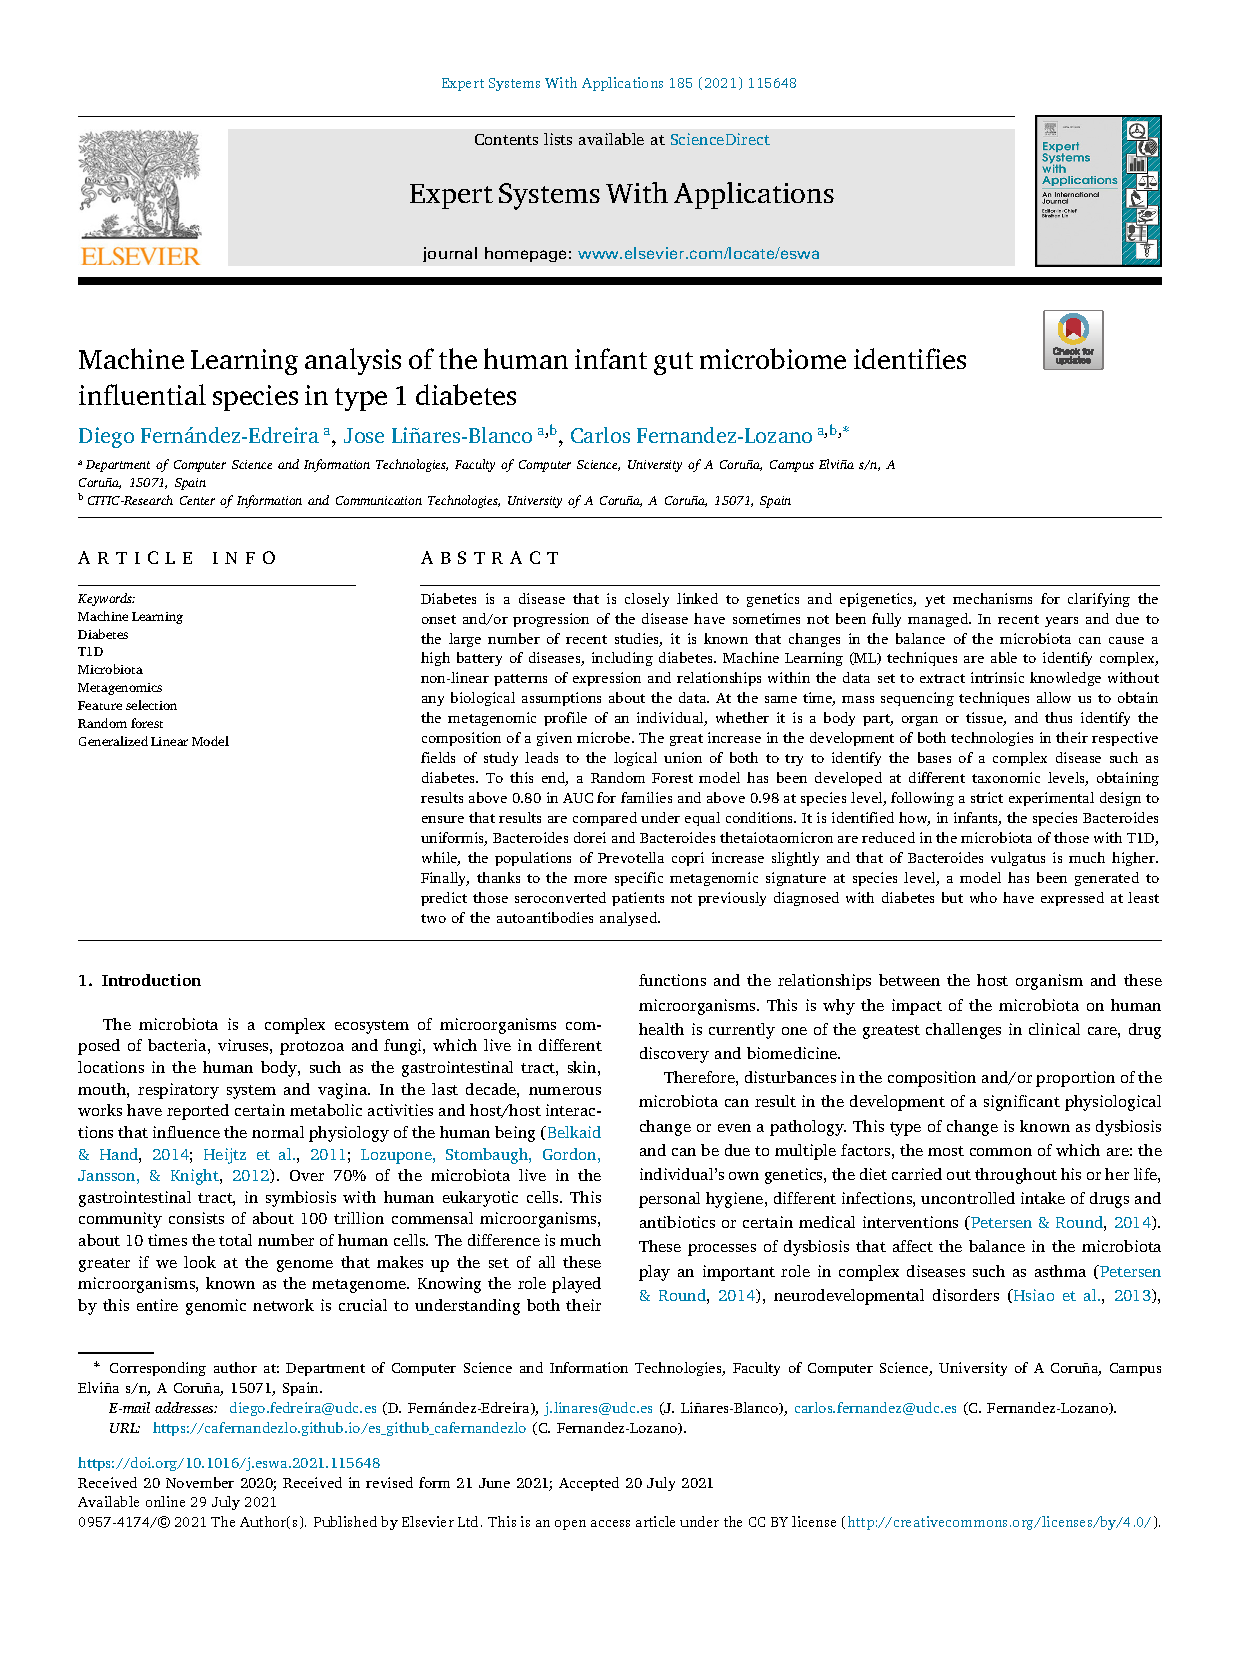
\includepdf[pages = -]{back/paper2}

\section{Caracterización del microbioma vaginal en el contexto de Vaginosis Bacteriana}

La VB es una de las infecciones más comunes en mujeres en edad reproductiva, pero su diagnóstico se ve complicado por la heterogeneidad de sus fenotipos y las respuestas variables al tratamiento. Un enfoque metagenómico permite explorar la disbiosis subyacente a esta condición, abriendo la puerta a una mejor clasificación y, con ello, a tratamientos más personalizados. Por tanto, este último trabajo tuvo como objetivo mejorar la caracterización de los fenotipos de VB y enriquecer la clasificación de esta enfermedad. Para ello, se emplean 5 cohortes de microbioma vaginal depositadas en el ENA \cite{leinonen2010european}.

Para realizar la caracterización y el subtipado de pacientes, se partió de una cohorte formada por casi 400 pacientes \cite{ravel2011vaginal}. Se utilizó el método de \textit{clustering} por consenso CCP \cite{wilkerson2010consensusclusterplus} para la división de los pacientes según sus perfiles microbianos. Como resultado, se definieron 4 subtipos (VCS I-IV), los cuales se comprobaron y validaron en el resto de las cohortes. Estos subtipos se emplearon para entrenar un modelo de tipo \textit{Elastic Net}, denominado VIBES (https://mall-lab.github.io/VIBES-docs/), capaz de generalizar en cohortes externas y distribuido como paquete en R. A partir de una firma metagenómica predefinida, VIBES estima la probabilidad de pertenencia de cada paciente a los distintos subtipos, lo que permite analizar sus puntuaciones en cohortes independientes. Finalmente, para comprobar la significancia biológica de los subgrupos obtenidos a través de VIBES, se realizó una comparación con un método de estratificación reconocido en el estado del arte, llamado VALENCIA \cite{france2020valencia}. Además de una comparación de subgrupos, se llevó a cabo un experimento para determinar si, integrando la información de ambos enfoques, se puede mejorar la predicción de un medicamento para VB, en comparación con usar ambos enfoques por separado.

Estos cuatro subgrupos están conformados por 20 especies, siendo taxones clave varias especies del género \textit{Lactobacillus}, y especies como \textit{Gardnerella vaginalis} y \textit{Atopobium vaginae}, entre otras. Posteriormente, se realizó una comparación con los subgrupos (CSTs) de VALENCIA, y resulta interesante observar que el subconjunto asintomático en VALENCIA se correspondió predominantemente al grupo VCS-I en nuestro análisis (caracterizado por mayores abundancias de \textit{Lactobacillus crispatus}). No obstante, también se identificaron diferencias significativas entre los dos sistemas de clasificación. En concreto, los grupos intermedios de VIBES, como VCS-II y VCS-III, muestran una gran heterogeneidad en comparación con los subtipos de CST. Esta discrepancia podría ser un indicador de que nuestro enfoque proporciona información adicional a VALENCIA. Finalmente, para comprobar la utilidad de VIBES (y medir su diferencia con VALENCIA en un caso práctico), se planteó la hipótesis de usar las variables obtenidas por ambos enfoques para predecir la respuesta al metronidazol mediante modelos de ML. Se observó que, al integrar la información de ambos enfoques, se logra un rendimiento de 0,76 de \textit{accuracy}, mejorando el rendimiento que se consigue usando enfoques individuales (0,7 de \textit{accuracy}), lo que indica que VIBES estaría captando información biológica complementaria a VALENCIA.


En conclusión, la identificación de los cuatro subgrupos VCS I-IV mediante el enfoque de \textit{clustering} por consenso enriquece la comprensión de la diversidad microbiana en el ecosistema vaginal. La comparación de los grupos obtenidos con este enfoque frente a los que se obtienen usando VALENCIA sugiere que nuestro enfoque proporciona información adicional y complementaria. Además, los resultados obtenidos al integrar ambos enfoques en la predicción de la respuesta al metronidazol evidencian este hecho. Estos hallazgos no solo contribuyen a la evaluación y al manejo de la VB, sino que también abren nuevas vías para la investigación de estrategias terapéuticas más adaptadas a las características individuales de cada paciente.

El código fuente para reproducir todos los análisis, junto con la documentación, está disponible en GitHub (https://github.com/MALL-Lab/VIBES-analysis). El modelo VIBES está disponible en GitHub (https://github.com/MALL-Lab/VIBES). Los datos de secuenciación de todas las cohortes (SRA022855, SRA051298, PRJNA208535, PRJNA797778 y PRJNA302078) pueden consultarse a través de sus respectivos números de acceso en el ENA.

Fui coautor principal del trabajo. Realicé el tratamiento y preprocesamiento de los datos, ejecuté la metodología de ML, construí las figuras y las tablas, y escribí el manuscrito. La información de participación de los otros autores está descrita en el artículo.

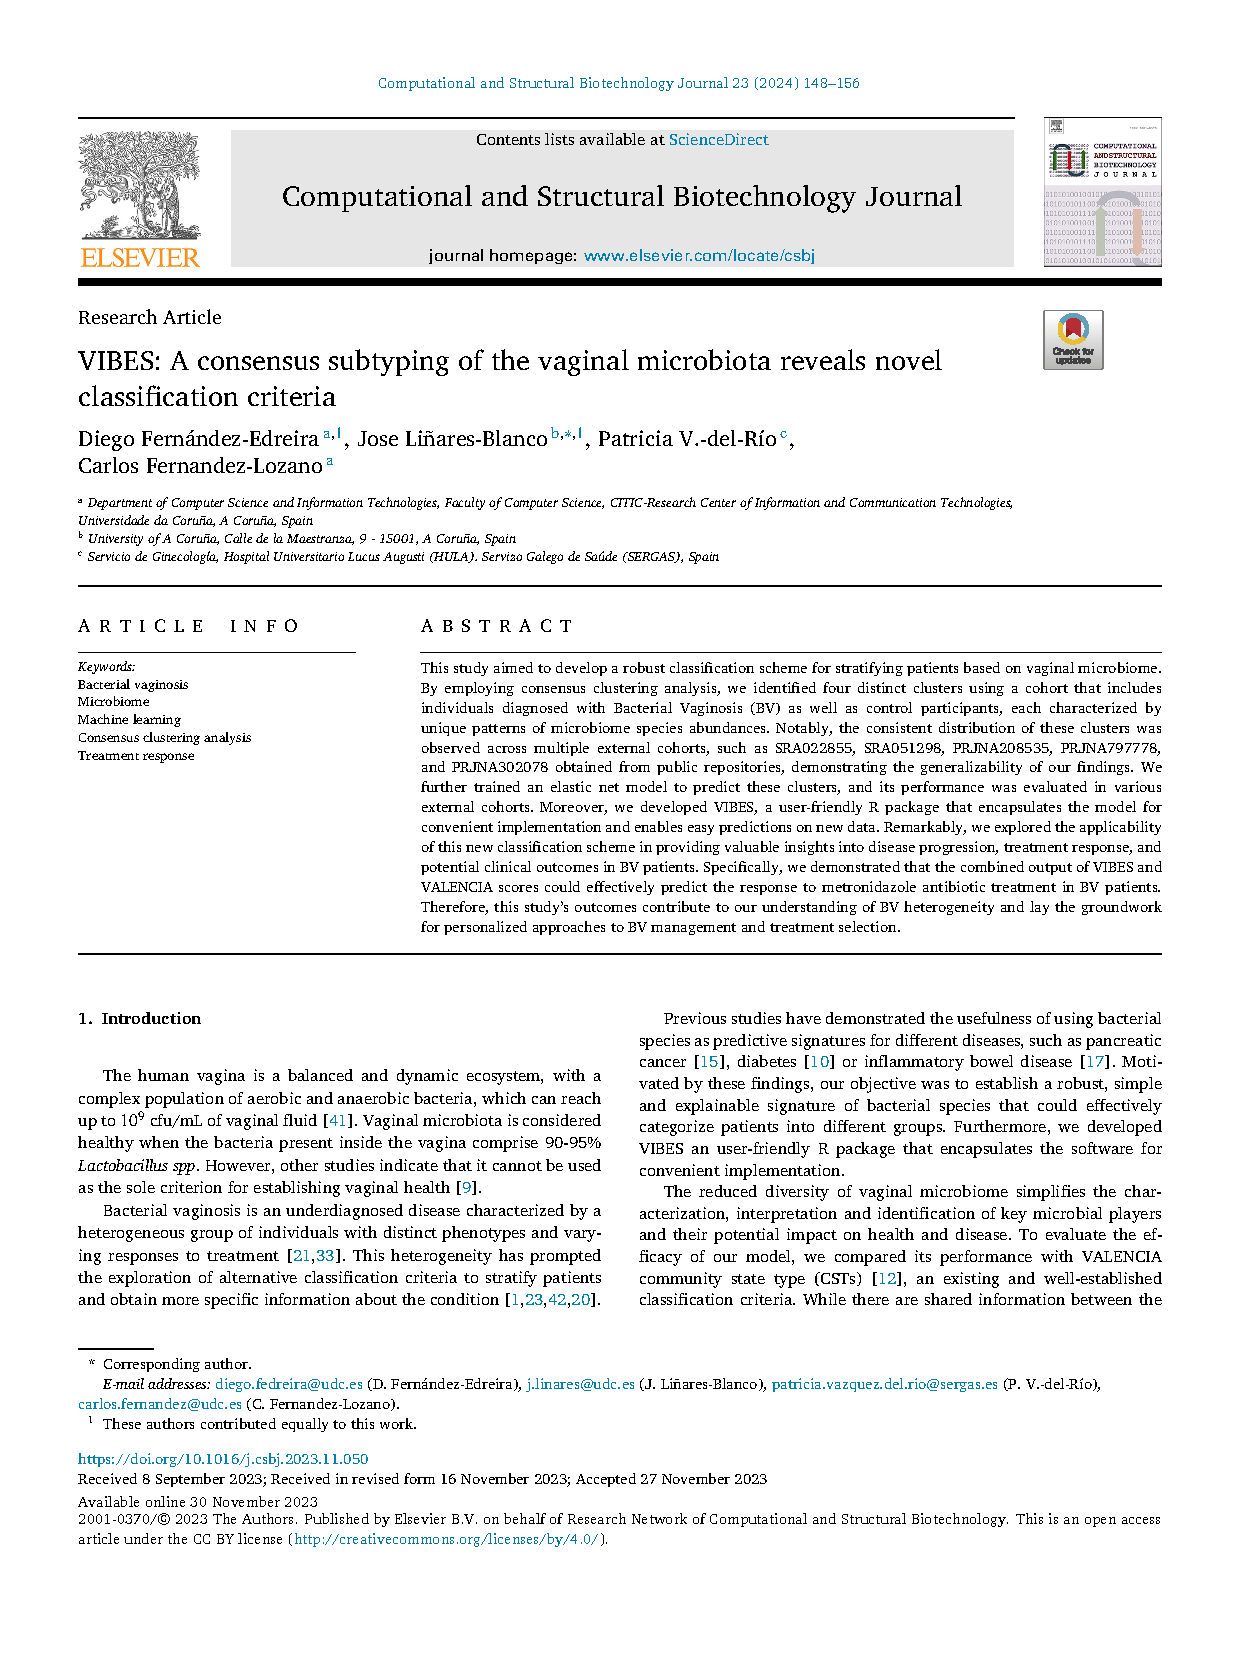
\includepdf[pages = -]{back/paper3}